\documentclass[12pt, a4paper]{article}

\makeatletter
\begingroup\endlinechar=-1\relax
       \everyeof{\noexpand}%
       \edef\x{\endgroup\def\noexpand\homepath{%
         \@@input|"kpsewhich --var-value=HOME" }}\x
\makeatother

\def\overleafhome{/tmp}% change as appropriate
\usepackage{indentfirst}
\usepackage{fontspec}
\ifx\homepath\overleafhome
\setmonofont{CONSOLA.TTF}[
BoldFont=CONSOLAB.ttf,
ItalicFont=CONSOLAI.ttf,
BoldItalicFont=CONSOLAZ.ttf
]
\else
\setmonofont{Consolas}
\fi

\usepackage{forest}
\usetikzlibrary{arrows.meta, angles}
\forestset{
  tree angle/.style={
    tikz={\path () coordinate (A) -- (!u) coordinate (B) -- (!n) coordinate (C) pic [draw] {angle};}
  }
}

\usepackage{algorithm}
\usepackage{algorithmic}
\usepackage{hyperref}
\hypersetup{
unicode=true,          % non-Latin characters in Acrobat’s bookmarks
pdftitle={},    % title   
%pdfauthor={爱让一切都对了},     % author   
%pdfcreator={爱让一切都对了},
%pdfproducer={OpenOffice.org 3.3},
breaklinks=true,
colorlinks=true,       % false: boxed links; ture: colored links
linkcolor=blue,          % color of internal links   
citecolor=blue,        % color of links to bibliography  
filecolor=magenta,      % color of file links   
urlcolor=cyan,           % color of external links  
}
\usepackage{xcolor}

\usepackage{url}
\def\UrlBreaks{\do\A\do\B\do\C\do\D\do\E\do\F\do\G\do\H\do\I\do\J\do\K\do\L\do\M\do\N\do\O\do\P\do\Q\do\R\do\S\do\T\do\U\do\V\do\W\do\X\do\Y\do\Z\do\[\do\\\do\]\do\^\do\_\do\`\do\a\do\b\do\c\do\d\do\e\do\f\do\g\do\h\do\i\do\j\do\k\do\l\do\m\do\n\do\o\do\p\do\q\do\r\do\s\do\t\do\u\do\v\do\w\do\x\do\y\do\z\do\0\do\1\do\2\do\3\do\4\do\5\do\6\do\7\do\8\do\9\do\.\do\@\do\\\do\/\do\!\do\_\do\|\do\;\do\>\do\]\do\)\do\,\do\?\do\'\do+\do\=\do\#}

\usepackage{listings}
\lstset{
%  %行号
%  %numbers=left,
%  %背景框
%  %framexleftmargin=10mm,
%  %frame=none,
%  %背景色
%  %backgroundcolor=\color[rgb]{1,1,0.76},
%  %样式
  keywordstyle=\color{blue}\bfseries,
%  identifierstyle=\bf,
%  numberstyle=\color[RGB]{0,192,192}, %行号的样式
  commentstyle=\it\color[RGB]{0,96,96},
  stringstyle=\rmfamily\slshape\color[RGB]{128,0,0},
%  %显示空格
%  %showstringspaces=false,
  basicstyle=\ttfamily\footnotesize, %修正大写字母间距过小
  columns=flexible, %修正大写字母间距过小
  breaklines=true, %对过长的代码自动换行
%  escapechar=!,
%  morekeywords={BEGIN}
    upquote=true,
  language=python
}

\newcommand{\code}[1]{\texttt{#1}}

\title{CS 188 Project Design Document}
\author{Weikeng Yang\\405346443 \and
Yingzhe Hu\\505366341 \and
Qiqi Gu\\604253019 \and
Dongyao Liang\\705313832 \and
Shuhua Zhan\\705190671}
\date{Team name: Random\\[2mm]January 24, 2020}

\usepackage[numbers]{natbib}
\setcitestyle{square}

\usepackage{graphicx}

\begin{document}

\maketitle

\section{The purpose of the software}
The project is a website searching apps on Google Play. The purpose of the software is to enhance the searching and filtering functions on Google Play so that users are able to filter apps by their permissions, whether they have ads, whether they have in-app purchase, free or paid, etc. Further, our website is able to sort apps by the number of permissions, price, stars, downloads, and sort of metrics to facilitate use case “search free sqlite database app with no ads with only storage read/write permissions, sorted by rating”.

\section{The architecture of the software}
In order to gather the app information, we have a web scraper which scrapes app information, including app name, categories, permissions, whether it contains ads, install fees, etc. and saves the data into database. 

To provide the search function, we must implement a web server. The web server renders a search box, where users can type in their keywords. Once they click the search button, the web page will show the list of apps matching the criterion. Figure \ref{fig:search-interface} shows the current web page where we are still adding filtering functions.

\begin{figure}[ht]
\centering
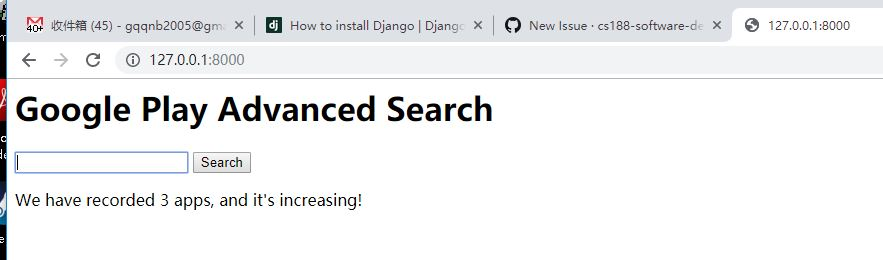
\includegraphics[width=0.8\textwidth]{search-interface.jpg}
\caption{The web page}
\label{fig:search-interface}
\end{figure}

\section{Components}
\subsection{Web Scraper}
Web Scraper is currently implemented with the help of the Python scrapy package\textsuperscript{\cite{scrapy}}. scrapy is a web scraper framework that uses Twisted reactor\textsuperscript{\cite{reactor}} to handle event loops because scrapy has events like parse response, \code{permissions\linebreak[2]\_retrieved}, \code{process\_item}, \code{open\_spider}, etc.

\code{AppInfoSpider.parse} is an event raised with parameter \code{response}, which is the HTML source code of the app detail page on Google Play. We choose proper CSS selectors or XPath selectors to scrape the app information. For instance, CSS selector \code{h1[itemprop=name]} selects the app name "Sonic the Hedgehog™ Classic" on \url{https://play.google.com/store/apps/details?hl=en&id=com.sega.sonic1px}.

SQLite3 support is part of python3 standard library.\textsuperscript{\cite{python-sqlite}}For simplicity, we choose to use sqlite3 as our database. Its query parameterization only works for the \code{where} clause.\textsuperscript{\cite{sqliteC++}}

\begin{figure}[ht]
\centering
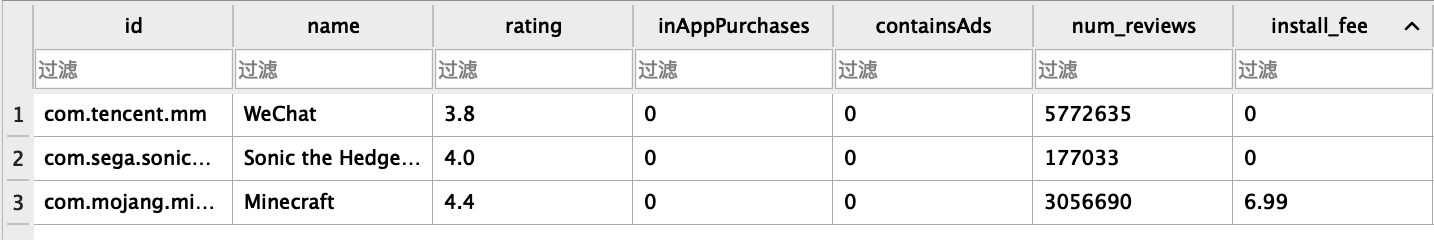
\includegraphics[width=0.8\textwidth]{critical_information.png}
\caption{Table Rows and Columns in SQLite}
\label{fig:critical-information}
\end{figure}

For now, our team has scraped 5 elements of information from Google Play Website, which are \code{rating}, \code{inAppPurchases}, \code{containAds}, \code{num\linebreak[4]\_reviews}, \code{install\_fee}, and a list of permissions. \code{rating} indicates the rating score of the apps; \code{inAppPurchases} indicates whether users are required to purchases products or pay fees inside the apps; \code{containAds} returns whether or not the apps have advertisements; \code{num\linebreak[2]\_reviews} returns the review comments from Google Play for the specific searched app; \code{install\_fee} returns the price of the apps and if it’s free, the value would be 0. Permissons are dynamically added to our table as a new column if we have never seen it before because we don't know all permissions an app can possibly have. Value of the permission columns would be 1 or 0, indicating if an app needs that permission.

\subsection{Website}
The website is built with python package django\textsuperscript{\cite{django}}. Listing \ref{lst:pattern-matching} is django URL pattern matching code that says if the path of the URL is empty, eg. \url{http://localhost:8080/}, the request shall be handled by \code{view.index()}. Once user submits a search request, in the proper request handler, we will use the keyword to search our database, or ask the scraper to update the database from Google Play, then return the result.

\begin{lstlisting}[frame=tb, caption=urls.py, label=lst:pattern-matching]
urlpatterns = [
    url(r'^$', view.index),
]
\end{lstlisting}

The website doesn't need to modify the database. Ideally it should open the database in read-only mode, but django doesn't support this. Considering the data in our database are not confidential, we are fine with opening the SQLite database with full permission.

\section{System Model}

\begin{figure}[ht]
\centering
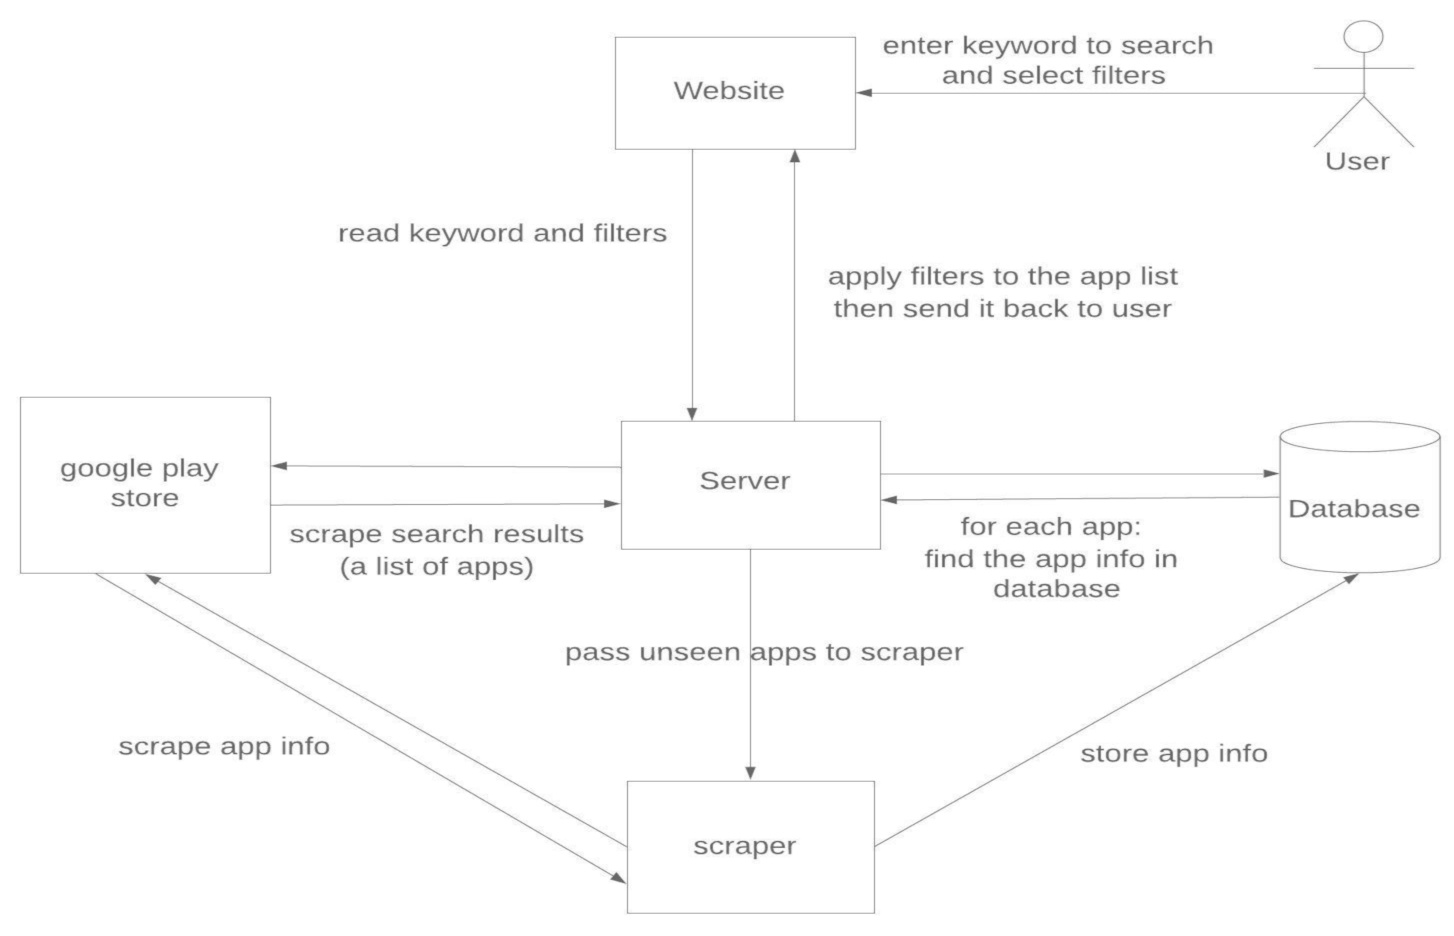
\includegraphics[width=\textwidth]{Context_Diagram.jpeg}
\caption{Design Diagram}
\label{fig:design_diagram}
\end{figure}



Use case:

\begin{enumerate}
    \item An user wants to search an boat game. He will type in keyword “boat”, select “Game” category and add the filters he wants (eg. free, rating>4.5, no Ads...)
    \item Our server uses the keyword and category to send a request to Google play store.
    \item Google play store will response us with a page that has a list of apps that match the keyword and the category. 
    \item we grab the app urls, then run the logic in Listing \ref{fig:database-step}.
    \item apply filters
    \item send back the filtered app list to user (see figure  \ref{fig:search_result}).
\end{enumerate}

\begin{algorithm}
    \caption{Pseduo-code for after searching an app}
    \label{fig:database-step}
\begin{algorithmic}
    \FOR{each app}
    \IF{app in our database}
    \STATE read app information
    \ELSE
    \STATE run our AppInfoSpider to scrape the app information from google play store
    \STATE put it in database
    \ENDIF
    \ENDFOR
\end{algorithmic}
\end{algorithm}
    

\begin{figure}[ht]
\centering
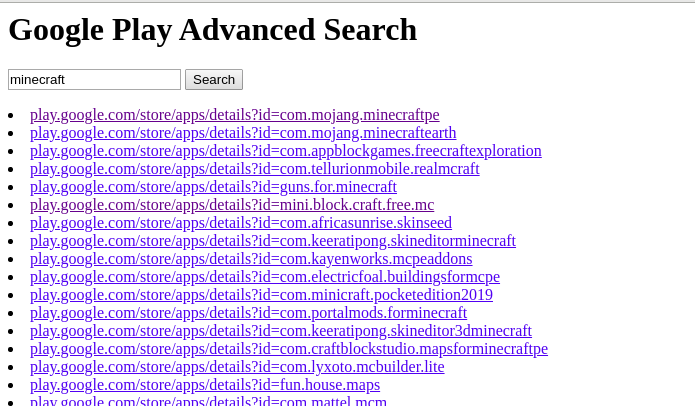
\includegraphics[width=1\textwidth]{homepage.png}
\caption{search result}
\label{fig:search_result}
\end{figure}

\section{Hardware and Software}
\subsection{Hardware}
We will rent a server from Google Cloud/AWS with reasonable storage and cores to host our application.

\subsection{Software}
The web scraper and the website are written in Python 3.7, as Python 2 is out of official support. The database is SQLite3 for now. The external python packages are recorded in \code{requirements.txt}, as seen in Listing \ref{lst:packages}.

We checked on \url{https://www.cvedetails.com/version/240190/Python-Python-3.7.html} that Python 3.7 has no major security issues.

\lstinputlisting[language={},frame=tb, caption=requirements.txt, label=lst:packages]{
\ifx\homepath\overleafhome
requirements.txt
\else
../../requirements.txt
\fi}

The whole piece of the software is runnable on both Linux and Windows system, but we will deploy it on Ubuntu 18.04 LTS.


\section{Security Requirements and Issues}

\begin{figure}[ht]
\centering
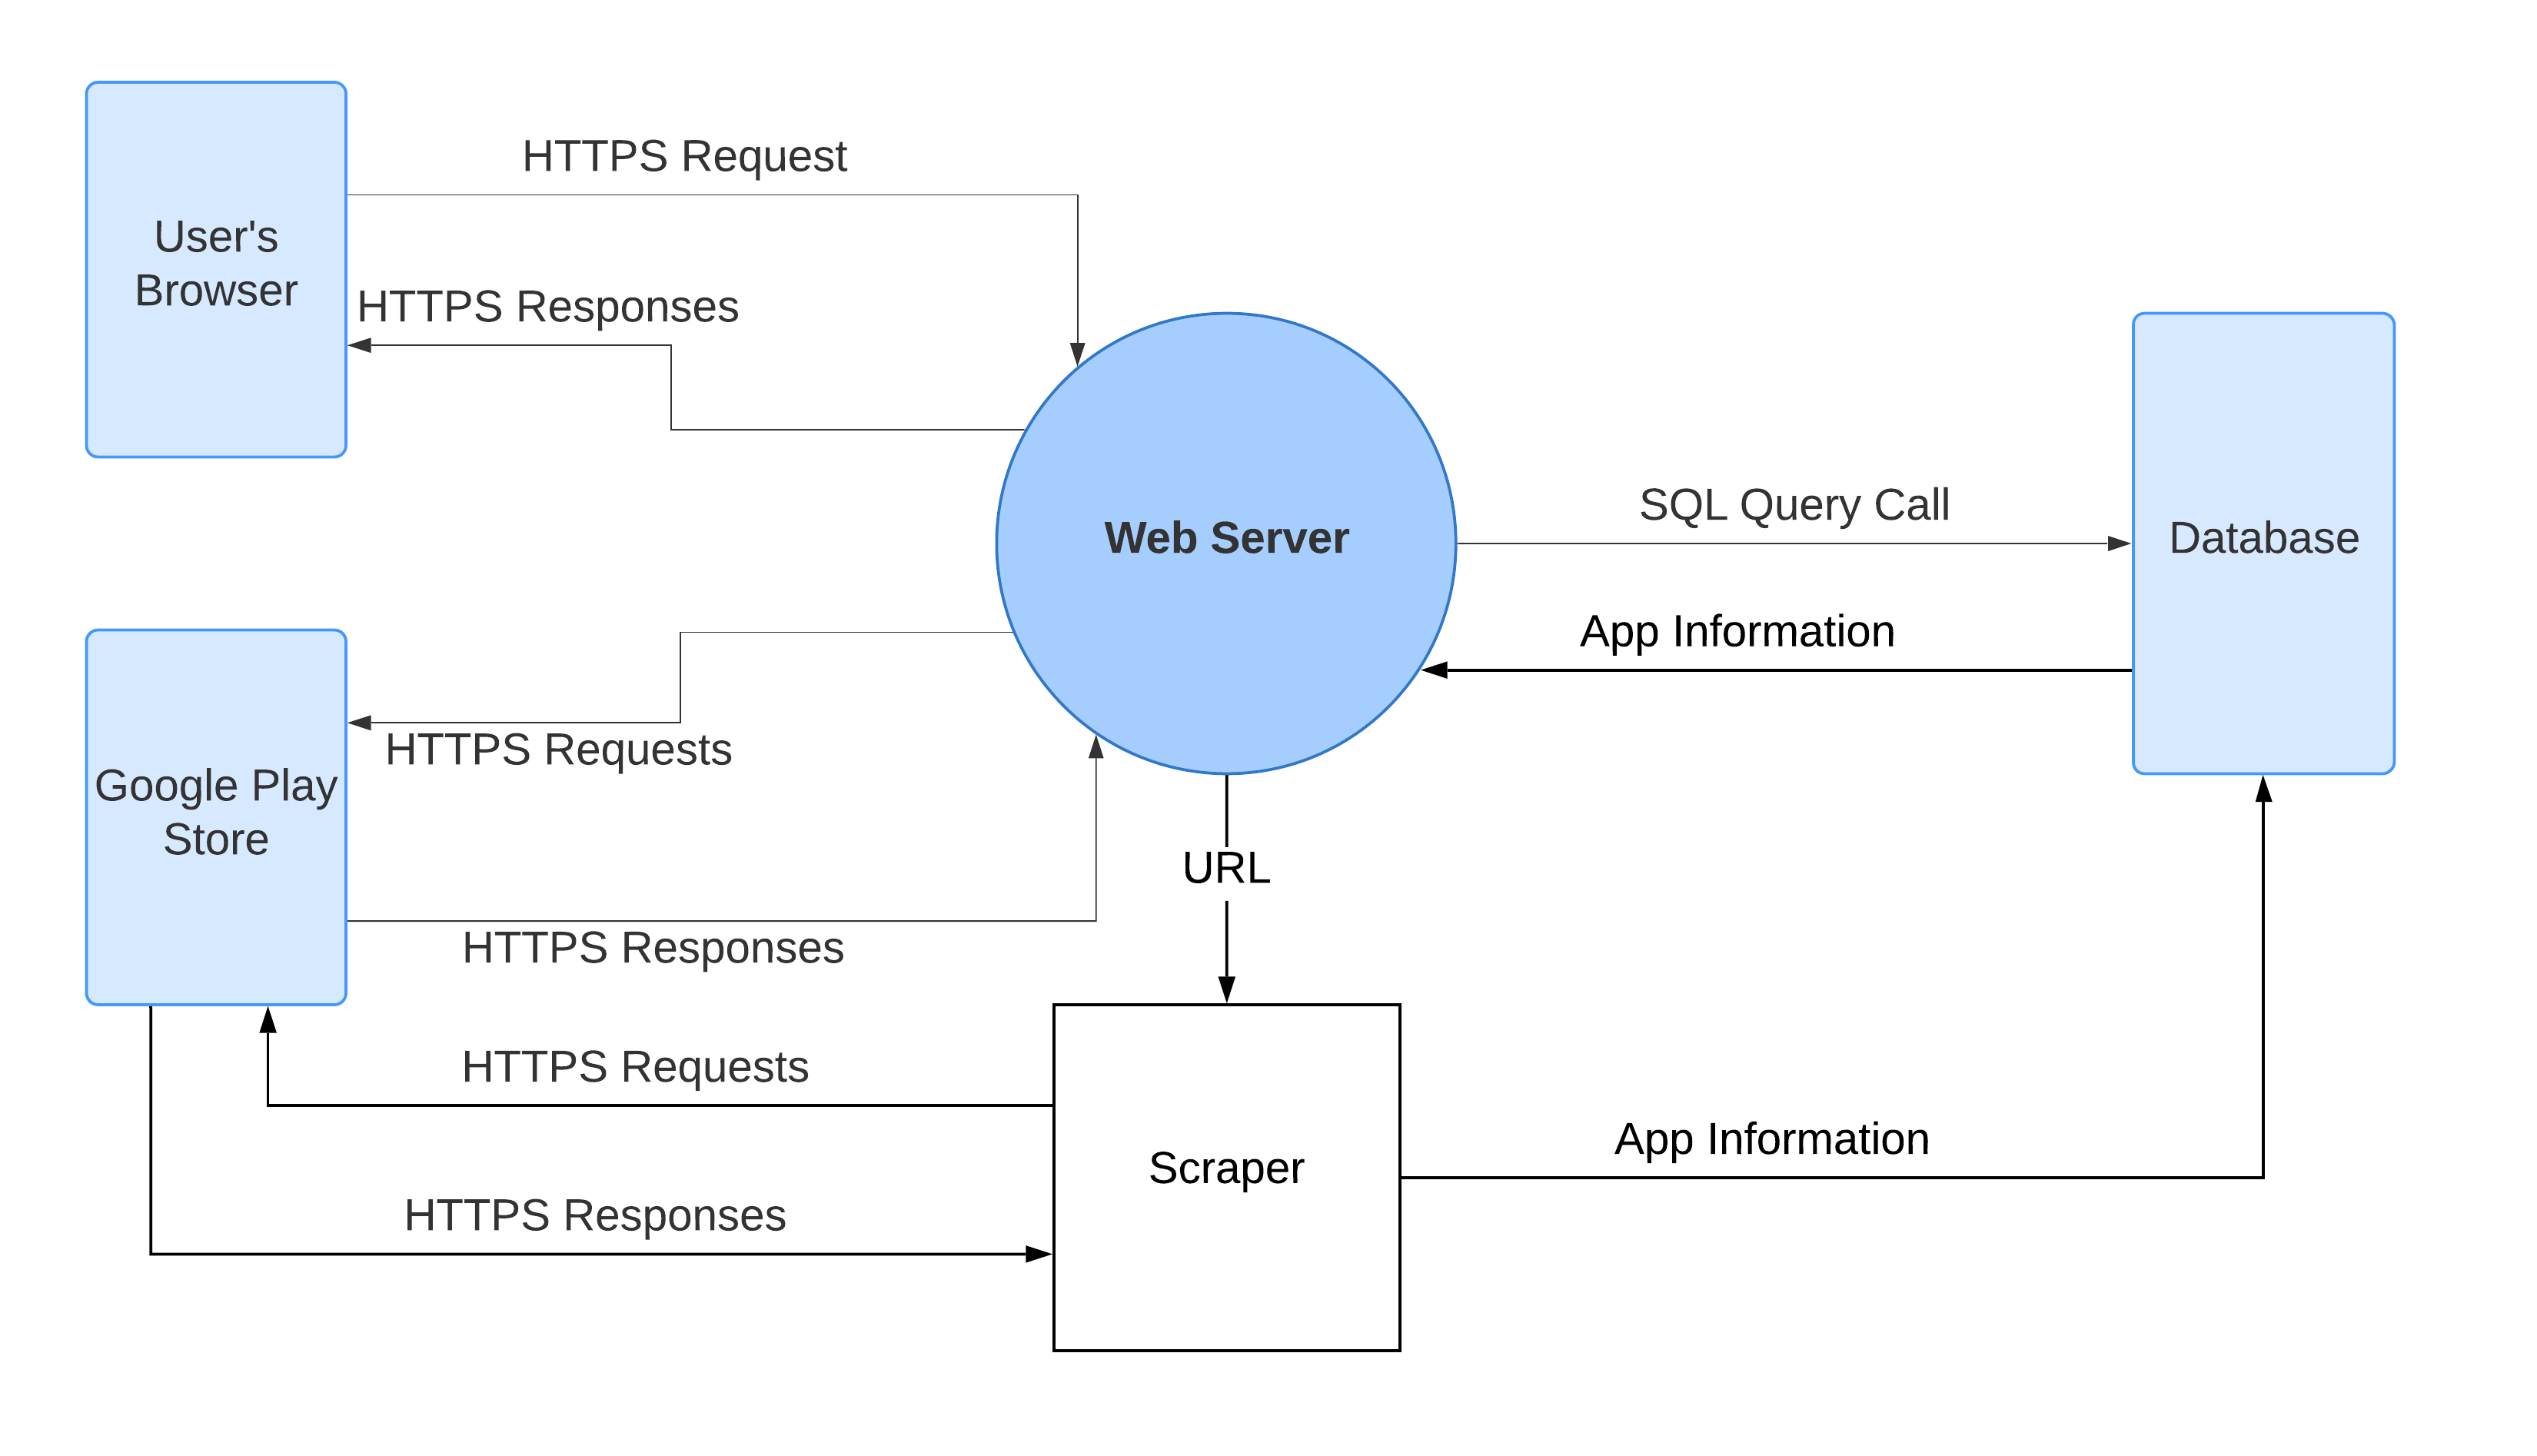
\includegraphics[width=1\textwidth]{Data_Flow_Diagram.png}
\caption{Data Flow Diagram}
\label{fig:Data_Flow}
\end{figure}

\subsection{Mitigate Denial-of-service Attack}
Denial-of-service Attack is a threat to our application. When facing a DOS threat, the victim may be attacked by a significant amount of incoming traffic from different sources so that the service of a website becomes unavailable. For example, an attacker might start a malicious activity by gathering the use of thousands of devices over the Internet to send a devastating number of unwanted packets to a website, which usually would be either large packets containing tons of data or sending large amount of small packets individually at the same time, making the website function much slower than usual or even out of service. For our product, it might not have to be a malicious activity from outside attackers but can also be that our website having an unexpected large number of users trying to search simultaneously, the server of our website might not be able to handle that.
Figure \ref{fig:dos} illustrates the attack tree .

In order to mitigate DOS attack, our team have come up with several possible solution which can be applied into our future development when building our website. One of them is that our application may impose a rate limit, for instance, an IP address can only send 10 search requests every 1 minute. If s/he reaches the limit, our website should show a warning. If s/he continues sending requests, we should block the IP through Linux firewall.

\begin{figure}[ht]
    \centering
    \begin{forest}
  for tree={
    draw,
    edge={-{Stealth[]}},
    l sep+=7.5pt,
    align=center,
  },
  [DOS Attack
    [Attack internally\\from the server
        [Gain access \\to the server]
    ]
    [Send massive requests\\from outside
        [Attacker gets\\many bots, tree angle]
        [server firewall\\is down
            [Gain access \\to the server]
        ]
    ]
    [Sends requests\\causing long execution
        [Find a bug in\\ our application]
    ]
  ]
\end{forest}

    \caption{Attack tree for DOS Attack}
    \label{fig:dos}
\end{figure}


\subsubsection{Prevent Arbitrary Code Execution}
We must not allow attackers to inject their code to our website and our website runs or sends the code to visitors to run. Figure \ref{fig:arbitrary-code-execution} illustrates the attack tree.

SQL Injection is a usually way to inject code. For example, our website has a search box and an attack may input some SQL update statement. If our database accidental executes the update statement, the database gets modified. If our website renders the injected data as HTML, it will execute on user's browser.

To prevent SQL injection, we use SQL parameterization when running SQL statements. In places where SQL parameterization is not supported, user input should be checked to ensure the security of data input. For example, single quotation marks, double quotation marks, colons and other characters should be converted or filtered.

What's more, it's possible that an attacker performs man-in-the-middle attack that hijacks the session between our server and Google Play. Google Play is using HTTPS so every time we scrape Google Play, we should check if the certificate is valid.

Our website needs to render app data as text instead of as HTML so that even if app data contains valid HTML, they will not execute on user's browser.

\begin{figure}[ht]
    \centering
    \begin{forest}
  for tree={
    draw, %框起来
    edge={-{Stealth[]}},
    l sep+=7.5pt, %vertical space between node and its parent.
    align=center,
  },
  [Run arbitrary code on our web page
    [Code injected to database, tree angle
        [Attacker gains\\direct access\\ to database]
        [The code\\ is from\\ Google Play
            [Attacker bypasses\\Google Play\\security check]
            [Man-in-the-middle\\attack on\\Google Play]
        ]
        [The code is\\from web search\\ interface
            [Database\\is writable, tree angle]
            [SQL\\paramertization\\failed]
        ]
    ]
    [Website treats\\the code as HTML]
  ]
\end{forest}
 \caption{Attack tree for arbitrary code execution}
   \label{fig:arbitrary-code-execution}
    
\end{figure}


\subsection{Prevent Cross-site request forgery (CSRF)}
It can steal or manipulate customer sessions and cookies, which can be used to impersonate a legitimate user, enabling hackers to view or change user records and execute transactions as that user.

Solution: 

Check the HTTP header refer information - After the Server receives the request, it can check the header and accept only the request from the local domain and ignore the request from the external domain.

Determine the type of HTTP request - Use \code{request.getMethod()} to determine whether the request is posted.

\subsection{Support HTTPS Communication}
When we develop the application, we test it with http://localhost. We shall make sure the application support HTTPS communication as our production server will enable HTTPS. 

In addition, we may enable OCSP Stapling. %补充一下

We may not enable HTTP Strict Transport Security because it requires our website to always have a valid certificate. We don't have enough manpower to maintain it.



\newcommand{\citeWeb}[3]{#1, \url{#2}, Retrieved #3.}


\begin{thebibliography}{99}
	\bibitem{scrapy} \citeWeb{Scrapy | A Fast and Powerful Scraping and Web Crawling Framework}{https://scrapy.org/}{2020-01-21}
	\bibitem{reactor} \citeWeb{Reactor Overview}{https://twistedmatrix.com/documents/current/core/howto/reactor-basics.html}{2020-01-21}
    \bibitem{django} \citeWeb{The Web framework for perfectionists with deadlines | Django}{https://www.djangoproject.com}{2020-01-21}
    \bibitem{python-sqlite} \citeWeb{sqlite3 — Python 3.8.1 documentation}{https://docs.python.org/3/library/sqlite3.html}{2020-01-21}
    \bibitem{sqliteC++} \citeWeb{An Introduction To The SQLite C/C++ Interface}{https://www.sqlite.org/cintro.html}{2020-01-21} “Parameters may not be used for column or table names.”
\end{thebibliography}
\end{document}
